An amplifier has a dc gain of $10^5$ and poles at $10^5$ Hz , $3.16 \times 10^5$ Hz and $10^6$ Hz . Find the value of $H$, and the corresponding closed-loop gain, for which a phase margin of $45\degree$ is obtained. 

\begin{enumerate}[label=\arabic*.,ref=\theenumi]
\numberwithin{equation}{enumi}

\item Find $G(s)$.
\\
\solution For a 3-pole amplifier open loop transfer function is 
\begin{align}
G(s) = \frac{G_0}{\brak{1+\frac{s}{p_{1}}}\brak{1+\frac{s}{p_{2}}}\brak{1+\frac{s}{p_{3}}}}
\end{align}

where the Gain and Poles are listed in Table \ref{table:ee18btech11016_Table_1}.
%
\begin{table}[!ht]
\centering
\input{./tables/ee18btech11016_1.tex}
\caption{}
\label{table:ee18btech11016_Table_1}
\end{table}
%
Thus, 
\begin{align}
G\brak{f} &= \frac{G_{0}}{\brak{1+\j\frac{f}{f_{1}}}\brak{1+\j\frac{f}{f_{2}}}\brak{1+\j\frac{f}{f_{3}}}}\\
&= \frac{10^{5}}{\brak{1+\j\frac{f}{10^5}}\brak{1+\j\frac{f}{3.16\times10^{5}}}\brak{1+\j\frac{f}{10^6}}}
\label{eq:ee18btech11016_1}
\end{align}
%
\item Given that $PM = 45 \degree$, find the crossover frequency $f_c$.
%\item Find the loop gain expression ($G(s)H$) (H is constant in this question).
%\\
%\solution 
%\begin{align}
%GH = \frac{10^{5}}{\brak{1+\j\frac{f}{10^5}}\brak{1+\j\frac{f}{3.16\times10^{5}}}\brak{1+\j\frac{f}{10^6}}} . H
%\label{eq:ee18btech11016_2}
%\end{align}

%\item Find the PM and the crossover frequency.
%\\
%\solution  
Let $L(s) = G(s)H$ be the loop gain.  Then
\begin{align}
PM = 180\degree - \phase{L(f_c)}
\label{eq:ee18btech11016_pmdef}
\end{align}
where
\begin{align}
\abs{L(f_c)} = 1
\end{align}
From \eqref{eq:ee18btech11016_pmdef},
\begin{align}
\phase{L(f_c)} = -135 \degree
\end{align}

%$\abs{G(f)H}=1$
%The phase margin = $180\degree$ - $\phi(f_{c})$ where $f_{c}$ is the frequency where $\abs{G(f)H}=1$.It is required that the phase margin is $45\degree$ , so that :

%\begin{align}
%45\degree &=  180\degree - \phi(f_{c}) \implies \phi(f_{c})=-135\degree.
%\end{align}
%From \eqref{eq:ee18btech11016_2} 
\begin{multline}
\implies -135\degree = -\tan^{-1}\brak{\frac{f_{c}}{10^5}}
\\
-\tan^{-1}\brak{\frac{f_{c}}{3.16\times10^5}}-\tan^{-1}\brak{\frac{f_{c}}{10^6}}
\end{multline}
\begin{align}
\text{or, }f_{c} = 315 \, kHz.
\label{eq:ee18btech11016_fc}
\end{align}

\item Verify your result using a Bode plot.
\\
\solution  The following code  id used to verify the value of $f_{c}$ Fig. \ref{fig:ee18btech11016_1}

\begin{lstlisting}
codes/ee18btech11016/ee18btech11016_1.py
\end{lstlisting}
%
\begin{figure}[!h]
\centering
\includegraphics[width=\columnwidth]{./figs/ee18btech11016/ee18btech11016_resultbode.eps}
\caption{}
\label{fig:ee18btech11016_1}
\end{figure}

\item Find the value of H.\\
\solution 
%From \eqref{eq:ee18btech11016_2},The magnitude of the loop gain at this frequency $f_{c}$ is given by $\abs{G(f_{c})H}$ :
\begin{align}
\because \abs{L\brak{f_c}} = \abs{G(f_{c})H} &= 1,
\end{align}
{\small 
\begin{multline}
H\brak{\frac{10^5}{\sqrt{1+\brak{\frac{315\times10^3}{10^5}}^2}\sqrt{1+\brak{\frac{315\times10^3}{3.16\times10^6}}^2}\sqrt{1+\brak{\frac{315\times10^3}{10^6}}^2}}} 
\\
=1
\end{multline}
}
upon substituting from \eqref{eq:ee18btech11016_1}
and \eqref{eq:ee18btech11016_fc}
%
\begin{align}
\implies  H = 34.651\times10^{-6}
\end{align}

The following code provides the method to calculate the unit step response and the values of H,G(fc).
\begin{lstlisting}
codes/ee18btech11016/ee18btech11016_verifyingvalues.py
\end{lstlisting}
%\item Find the corresponding closed-loop gain for which a phase margin of $45\degree$ is obtained.\\
%\solution The closed loop dc gain is given as
%\begin{align}
%A_{f} = \frac{G_{0}}{1+HG_{0}}=\frac{10^5}{1+34.651\times10^{-6}(10^5)}
%\end{align} 
%\begin{align}
%A_{f} = 22.3957\times10^3
%\end{align}
%
%
\item Sketch the block diagram for the given closed loop  system with $PM = 45 \degree$. \\
\solution See Fig. 	\ref{fig:ee18btech11016_figa}.

\begin{figure}[ht!]
	\begin{center}
		\resizebox{\columnwidth/1}{!}{\input{./figs/ee18btech11016/ee18btech11016_figa.tex}}
	\end{center}
	\caption{}
	\label{fig:ee18btech11016_figa}
\end{figure}

%The transfer function of OPAMP is
%\begin{align}
%    G(s) = \frac{10^{5}}{\brak{1+\frac{s}{2\pi \times 10^5}}\brak{1+\frac{s}{2\pi \times3.16 \times 10^{5}}}\brak{1+\frac{s}{2\pi \times 10^{6}}}}
%\end{align}
%
\item Design the circuit for $H$\\
\solution In Fig. 	\ref{fig:ee18btech11016_figb},
%
\begin{align}
    H &= \frac{V_{f}}{V_{o}} = \frac{R_{f_{1}}}{R_{f_{1}}+R_{f_{2}}} \approx 34.651\times10^{-6}
\\
\implies 
\begin{split}
    R_{f_{1}} &= 100\ohm\\
    R_{f_{2}} &= 4.057M\ohm
\end{split}
\end{align}
\begin{figure}[ht!]
	\begin{center}
		\resizebox{\columnwidth/2}{!}{\input{./figs/ee18btech11016/ee18btech11016_figb.tex}}
	\end{center}
	\caption{}
	\label{fig:ee18btech11016_figb}
\end{figure}

%Choosing 
%\begin{align}
%    R_{f_{1}} = 100\ohm\\
%    R_{f_{2}} = 4.057M\ohm
%\end{align}
%\begin{align}
%H = \frac{R_{f_{1}}}{R_{f_{1}}+R_{f_{2}}} = \frac{100}{100+4.057\times10^6} \approx 34.651\times10^{-6}
%\end{align}
\item Design the feedback circuit using an OPAMP.
\\
\solution See Fig. 	\ref{fig:ee18btech11016_figc}

\begin{figure}[ht!]
	\begin{center}
		\resizebox{\columnwidth}{!}{\input{./figs/ee18btech11016/ee18btech11016_figc.tex}}
	\end{center}
	\caption{}
	\label{fig:ee18btech11016_figc}
\end{figure}

\numberwithin{figure}{enumi}
\item Simulate the circuit in ngspice.\\
\solution For $H=34.651\times10^{-6}$, the closed loop response is
\begin{align}
\abs T \approx \frac{1}{H} = 28.8588\times10^{3}
\label{eq:ee18btech11016_T}
\end{align}
%which can be observable from graph also.
%\\
The following code provides instructions about the simulation.
\begin{lstlisting}
codes/ee18btech11016/spice/README.md
\end{lstlisting}
%
The following netlist simulates the unity feedback system for a DC input
%
\begin{lstlisting}
codes/ee18btech11016/spice/ee18btech1016_sim.net
\end{lstlisting}
which is plotted using the following code in Fig. \ref{fig:ee18btech11016_spice}.  Note that the DC gain in Fig. \ref{fig:ee18btech11016_spice} is the same as \eqref{eq:ee18btech11016_T}

 \begin{lstlisting}
codes/ee18btech11016/spice/ee18btech11016_simulation.py
\end{lstlisting}
\renewcommand{\thefigure}{\theenumi.\arabic{figure}}
\begin{figure}[!h]
\centering
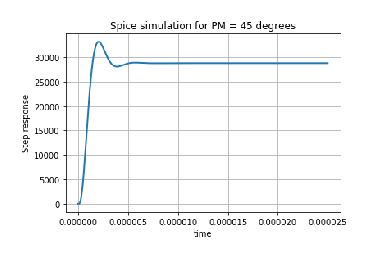
\includegraphics[width=\columnwidth]{./figs/ee18btech11016/ee18btech11016_spice.eps}
\caption{}
\label{fig:ee18btech11016_spice}
\end{figure}

%\item Overview of implementation.\\
%\solution 
Fig. \ref{fig:ee18btech110016_circuit_1} shows how the OPAMP circuit is actually implemented in spice using the parameters in Table \ref{table:ee18btech11016_Table_2}  

\begin{figure}[!ht]
	\begin{center}
				\resizebox{\columnwidth}{!}{\input{./figs/ee18btech11016/circuit_1.tex}}
	\end{center}
\caption{Circuit resembling G(s)}
\label{fig:ee18btech110016_circuit_1}
\end{figure}

\begin{table}[!ht]
\centering
\input{./tables/ee18btech11016_table2.tex}
\caption{}
\label{table:ee18btech11016_Table_2}
\end{table}
\renewcommand{\thefigure}{\theenumi}

\end{enumerate}
